\textbf{\underline{OZ 8 - LC- en  RLC-circuits - Oefening 2:}}
\vspace{0.5cm}

Een spoel met $820$ windingen heeft een weerstand van $24,0 \ \Omega$, en wordt geplaatst rond een solenoïde met $12500$ windingen van $7.00$ cm lang. Zowel de spoel als de solenoïde hebben een doorsnede van oppervlakte $1.00\cdot10^{-4} \ \text{m}^2$.

\vspace{0.3cm}
\begin{minipage}{.66\textwidth}
    \begin{enumerate}[(a)]
        \item 
            Hoe lang duurt het voordat de stroom door de solenoïde $63,2\%$ van zijn maximale waarde bereikt?
        \item 
            Bepaal de gemiddelde tegen-emf veroorzaakt door de zelfinductie van de solenoïde tijdens dit tijdsinterval,
        \item 
            de gemiddelde snelheid van verandering van het magnetische flux door de spoel tijdens dit tijdsinterval,
        \item 
            en de grootte van de gemiddelde geïnduceerde stroom in de spoel.
    \end{enumerate}
\end{minipage}
\begin{minipage}{.3\textwidth}
    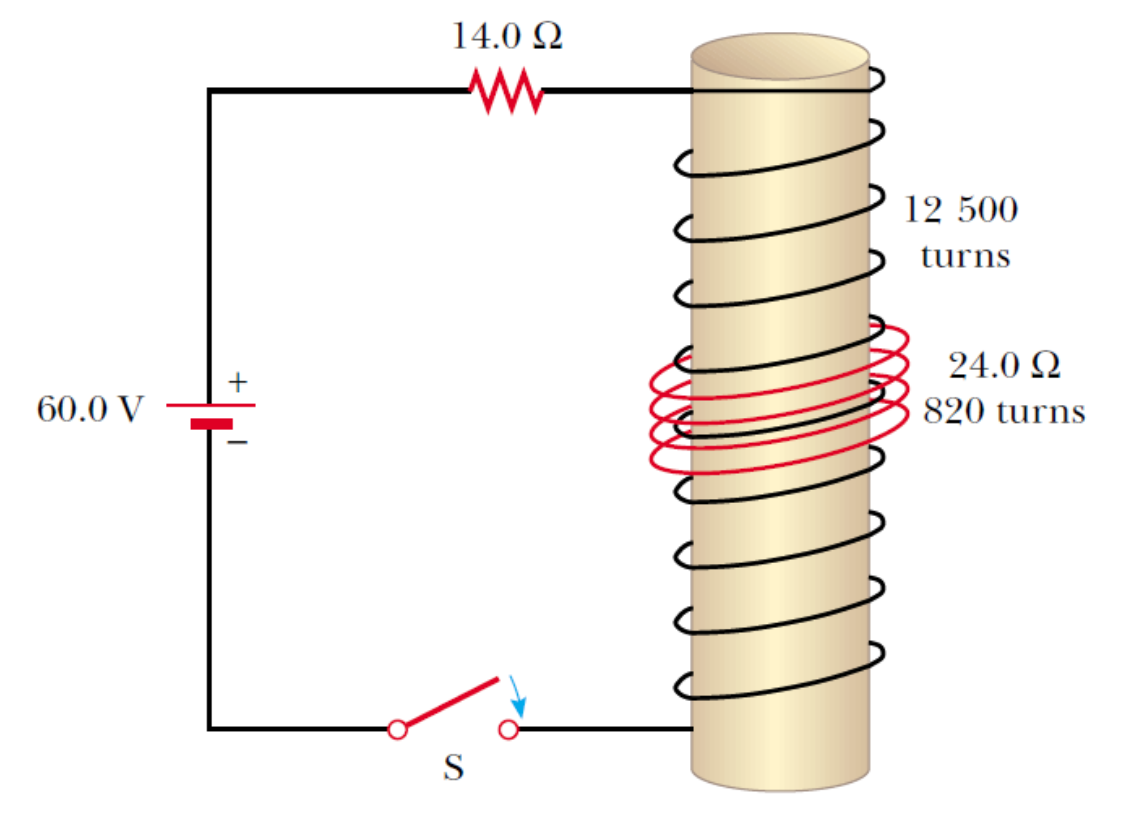
\includegraphics[scale = 0.3]{oz08/resources/Oz8Oef2.png}
\end{minipage}

\begin{description}[labelwidth=1.5cm, leftmargin=!]
    \item[Geg. :]   $N_1 = 820$, $X_1 = 24.0 \ \Omega$, $N_2 = 12500$, $\ell_2 = 7.00 \ \text{cm}$, $A_1 = A_2 = 1.00\cdot10^{-4} \ \text{m}^2$, $R = 14.0 \ \Omega$, $\Delta V = 60 \ \text{V}$
\end{description}

\begin{enumerate}[(a)]
    \item 
        \begin{description}[labelwidth=1.5cm, leftmargin=!]
            \item[Gevr. :] $t_{63.2\%}$ ?
            \item[Opl. :]  
                In een RL-kring volgt de stroom de volgende formule
                \begin{equation*}
                    I(t) = I_{\text{max}} \left( 1 - e^{-\frac{t}{\tau}} \right)
                \end{equation*}
                met $\tau = \frac{L}{R}$. De stroom bereikt $63.2\%$ van zijn maximale waarde wanneer $t = \tau $. We kunnen dus stellen dat
                \begin{equation*}
                    t_{63.2\%} = \frac{L_2}{R} = \frac{\mu_0N_2^2A_2}{\ell_2R}.
                \end{equation*}
                We berekenen nu triviaal de tijd door in te vullen:
                \begin{equation*}
                    t_{63.2\%} = 0.02 \ \text{s} \approx 20.0 \ \text{ms}.
                \end{equation*}


        \end{description}
    \item 
        \begin{description}[labelwidth=1.5cm, leftmargin=!]
            \item[Gevr. :] $\mathcal{E}_{\text{back}}$ ?
            \item[Opl. :]
                De gemiddelde geïnduceerde emf is gelijk aan 
                \begin{equation*}
                    \mathcal{E}_{\text{back}} = -L_2 \frac{\Delta I}{\Delta t}.
                \end{equation*}
                waarbij 
                \begin{equation*}
                    \frac{\Delta I}{\Delta t} = 0.632 \frac{\Delta I_{\text{max}}}{\Delta t} = 0.632 \frac{\Delta V}{R\Delta t}.
                \end{equation*}
                We kunnen nu de geïnduceerde emf berekenen:
                \begin{equation*}
                    \mathcal{E}_{\text{back}} = -L_2 \frac{\Delta I}{\Delta t} = -0.632 \frac{\mu_0N_2^2A_2}{\ell_2}\frac{\Delta V}{R\Delta t} = -37.9 \ \text{V}.
                \end{equation*}
        \end{description}
    \item 
        \begin{description}[labelwidth=1.5cm, leftmargin=!]
            \item[Gevr. :] $\frac{\Delta \Phi_B}{\Delta t}$ ?
            \item[Opl. :]   
                De gemiddelde snelheid van de verandering van het magnetische flux is gelijk aan 
                \begin{equation*}
                    \frac{\Delta \Phi_B}{\Delta t} = -\frac{\mathcal{E}_{\text{back}}}{N_2} \approx 3.04 \ \text{mV}.
                \end{equation*}
        \end{description}
    \item 
        \begin{description}[labelwidth=1.5cm, leftmargin=!]
            \item[Gevr. :] $I_{\text{ind}}$ ?
            \item[Opl. :]   
                De gemiddelde stroom is gelijk aan 
                \begin{equation*}
                    I_{\text{ind}} = \frac{\mathcal{E}_{\text{ind}}}{X_1} = \frac{N_1}{X_1}\frac{\Delta \Phi_b}{\Delta t} \approx 104 \ \text{mA}.
                \end{equation*}
        \end{description}
\end{enumerate}

\textbf{Opmerking:} in (b), (c) en (d) wordt er gevraagd achter het gemiddelde en niet ogenblikkelijke! 

\vspace{1cm}